\documentclass[tikz,
  margin=3pt,
  convert,
  convert={
    outext=.png,
    command=\unexpanded{
      pdftocairo -r 300 -png \infile % 将生成的pdf文件转换为png图像
    }
  }
  ]{standalone}

\usepackage{pgfplots}
\pgfplotsset{compat=newest}

\begin{document}
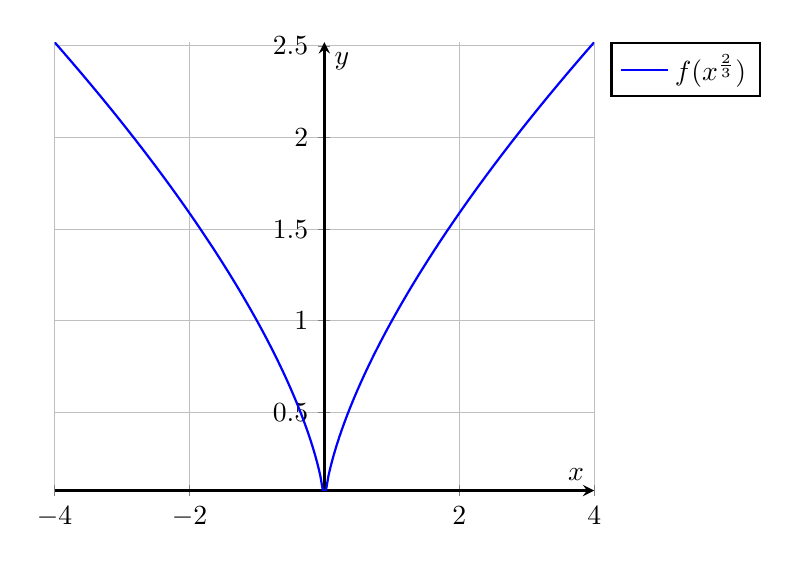
\begin{tikzpicture}
  \begin{axis}[
    xlabel={$x$},
    ylabel={$y$},
    axis lines=middle,
    samples=200,
    grid,
    thick,
    domain=-4:4,
    legend pos=outer north east,
    smooth,
    ]
    \addplot+[no marks]{abs(x)^(2/3)};
    \addlegendentry{$f(x^{\frac{2}{3}})$}
  \end{axis}
\end{tikzpicture}
\end{document}

%%% Local Variables:
%%% mode: latex
%%% TeX-master: t
%%% End:
